\subsubsection{Parâmetros arquitetônicos dos modelos genéricos}
\noindent A preparação para o início das simulações é precedida pela definição dos parâmetros arquitetônicos e das variáveis contidas em cada um destes. Com base no levantamento in loco e no referencial teórico, são inicialmente modificados os atributos arquitetônicos em três fases: envoltória, sistemas de iluminação e condicionamento de ar. As modificações foram implementadas de forma ordenada, a fim de evidenciar a influência de cada medida proposta no consumo final de energia elétrica da edificação genérica. As medidas propostas para analise por meio de simulação computacional estão apresentadas na Tabela \ref{tab:tabela10}.
\begin{table}[H]
    \small
    \caption{Zonas térmicas dos modelos genéricos.}%\vspace*{0.3cm}
    \label{tab:tabela10}
    \begin{tabular*}{\columnwidth}{@{\extracolsep{\fill}}clcrl}
    \hline
    \multicolumn{2}{c}{Parâmetros}                                                                                                                      & \multicolumn{2}{c}{Variáveis} & Descrição                                                                                                                                                                                                                                                                                                                                                                                                                                                                 \\ \hline
    \multicolumn{1}{c}{\multirow{4}{*}{1}} & \multirow{4}{*}{Orientação Solar}                                                                          & a          & 0°               & \multirow{4}{*}{\makecell[l]{Orientação solar da fachada \\principal.}}                                                                                                                                                                                                                                                                                                                                                                                                   \\
    \multicolumn{1}{c}{}                   &                                                                                                            & b          & 90º              &                                                                                                                                                                                                                                                                                                                                                                                                                                                                           \\
    \multicolumn{1}{c}{}                   &                                                                                                            & c          & 180º             &                                                                                                                                                                                                                                                                                                                                                                                                                                                                           \\
    \multicolumn{1}{c}{}                   &                                                                                                            & d          & 270º             &                                                                                                                                                                                                                                                                                                                                                                                                                                                                           \\ \hline
    \multirow{8}{*}{2}                     & \multirow{8}{*}{Vidro com baixo Fator Solar}                                                               &            &                  & \multirow{8}{*}{\makecell[l]{Foram simuladas duas \\situações aplicas aos modelos \\genéricos: a primeira utilizando \\o vidro levantado in loco \\(a) e o modelo mais eficiente \\comercializado no mercado \\brasileiro (b) (CB3E; \\ABIVIDRO, 2015).}}                                                                                                                                                                                                                   \\
                                           &                                                                                                            &            &                  &                                                                                                                                                                                                                                                                                                                                                                                                                                                                           \\
                                           &                                                                                                            & a          & FS: 0,44         &                                                                                                                                                                                                                                                                                                                                                                                                                                                                           \\
                                           &                                                                                                            &            &                  &                                                                                                                                                                                                                                                                                                                                                                                                                                                                           \\
                                           &                                                                                                            &            &                  &                                                                                                                                                                                                                                                                                                                                                                                                                                                                           \\
                                           &                                                                                                            & b          & FS: 0,16         &                                                                                                                                                                                                                                                                                                                                                                                                                                                                           \\
                                           &                                                                                                            &            &                  &                                                                                                                                                                                                                                                                                                                                                                                                                                                                           \\
                                           &                                                                                                            &            &                  &                                                                                                                                                                                                                                                                                                                                                                                                                                                                           \\ \hline
    \multirow{13}{*}{3}                    & \multirow{13}{*}{\makecell[l]{Percentual de Área de Abertura\\ da Fachada Total – PAF\textsubscript{T}}}   &            &                  & \multirow{13}{*}{\makecell[l]{As aberturas das fachadas foram \\definidas de acordo com as \\indicações de programas de \\economia de energia como \\PROCEL EDIFICA e o \textit{Advanced} \\ \textit{Energy Design Guide for Small} \\ \textit{to Medium Office Buildings} \\(Guia Avançado de Planejamento \\Energético para Edificações de \\Escritório de Pequeno e Médio \\Porte) da ASHRAE (ASHRAE \\et al., 2014, 2019; FERRADOR \\FILHO; AGUIAR; KNIESS, 2018).}}  \\
                                           &                                                                                                            &            &                  &                                                                                                                                                                                                                                                                                                                                                                                                                                                                           \\
                                           &                                                                                                            &            &                  &                                                                                                                                                                                                                                                                                                                                                                                                                                                                           \\
                                           &                                                                                                            & a          & 30\%             &                                                                                                                                                                                                                                                                                                                                                                                                                                                                           \\
                                           &                                                                                                            &            &                  &                                                                                                                                                                                                                                                                                                                                                                                                                                                                           \\
                                           &                                                                                                            &            &                  &                                                                                                                                                                                                                                                                                                                                                                                                                                                                           \\
                                           &                                                                                                            & b          & 50\%             &                                                                                                                                                                                                                                                                                                                                                                                                                                                                           \\
                                           &                                                                                                            &            &                  &                                                                                                                                                                                                                                                                                                                                                                                                                                                                           \\
                                           &                                                                                                            &            &                  &                                                                                                                                                                                                                                                                                                                                                                                                                                                                           \\
                                           &                                                                                                            & c          & 80\%             &                                                                                                                                                                                                                                                                                                                                                                                                                                                                           \\
                                           &                                                                                                            &            &                  &                                                                                                                                                                                                                                                                                                                                                                                                                                                                           \\
                                           &                                                                                                            &            &                  &                                                                                                                                                                                                                                                                                                                                                                                                                                                                           \\
                                           &                                                                                                            &            &                  &                                                                                                                                                                                                                                                                                                                                                                                                                                                                           \\ \hline
    \multirow{8}{*}{4}                     & \multirow{8}{*}{\makecell[l]{Sistema de Condicionamento \\de Ar}}                                          &            &                  & \multirow{8}{*}{\makecell[l]{Foram adotados para a simulação \\o sistema de condicionamento de \\ar observado em levantamento, \\sendo este o Sistema Central de \\Água Gelada (CAG), o sistema \\individual \textit{Split}, e o \textit{Variable} \\ \textit{Refrigerant Fluid–VRF} \\(CBCS, 2015).}}                                                                                                                                                                    \\
                                           &                                                                                                            & a          & CAG/Fancoil      &                                                                                                                                                                                                                                                                                                                                                                                                                                                                           \\
                                           &                                                                                                            &            &                  &                                                                                                                                                                                                                                                                                                                                                                                                                                                                           \\
                                           &                                                                                                            & b          & Split            &                                                                                                                                                                                                                                                                                                                                                                                                                                                                           \\
                                           &                                                                                                            &            &                  &                                                                                                                                                                                                                                                                                                                                                                                                                                                                           \\
                                           &                                                                                                            & c          & VRF              &                                                                                                                                                                                                                                                                                                                                                                                                                                                                           \\
                                           &                                                                                                            &            &                  &                                                                                                                                                                                                                                                                                                                                                                                                                                                                           \\
                                           &                                                                                                            &            &                  &                                                                                                                                                                                                                                                                                                                                                                                                                                                                           \\ \hline
    \multirow{6}{*}{5}                     & \multirow{6}{*}{\makecell[l]{Transmitância térmica da \\parede da envoltória}}                             & a          & 2,46 W/m²K       & \multirow{6}{*}{\makecell[l]{Valores de transmitância \\baseados Anexo Geral V – Catálogo \\de Propriedades Térmicas de \\Paredes, Coberturas e Vidros \\(INMETRO, 2013).}}                                                                                                                                                                                                                                                                                               \\
                                           &                                                                                                            &            &                  &                                                                                                                                                                                                                                                                                                                                                                                                                                                                           \\
                                           &                                                                                                            & b          &                  &                                                                                                                                                                                                                                                                                                                                                                                                                                                                           \\
                                           &                                                                                                            &            & 0,38 W/m²K       &                                                                                                                                                                                                                                                                                                                                                                                                                                                                           \\
                                           &                                                                                                            &            &                  &                                                                                                                                                                                                                                                                                                                                                                                                                                                                           \\
                                           &                                                                                                            & c          & 0,32 W/m²K       &                                                                                                                                                                                                                                                                                                                                                                                                                                                                           \\ \hline
    \multirow{6}{*}{6}                     & \multirow{6}{*}{\makecell[l]{Transmitância térmica da \\cobertura}}                                        & a          & 3,73 W/m²K       & \multirow{6}{*}{\makecell[l]{Valores de transmitância \\baseados Anexo Geral V – Catálogo \\de Propriedades Térmicas de \\Paredes, Coberturas e Vidros \\(INMETRO, 2013).}}                                                                                                                                                                                                                                                                                               \\
                                           &                                                                                                            &            &                  &                                                                                                                                                                                                                                                                                                                                                                                                                                                                           \\
                                           &                                                                                                            & b          & 0,55 W/m²K       &                                                                                                                                                                                                                                                                                                                                                                                                                                                                           \\
                                           &                                                                                                            &            &                  &                                                                                                                                                                                                                                                                                                                                                                                                                                                                           \\
                                           &                                                                                                            &            &                  &                                                                                                                                                                                                                                                                                                                                                                                                                                                                           \\
                                           &                                                                                                            &            &                  &                                                                                                                                                                                                                                                                                                                                                                                                                                                                           \\ \hline
    \multicolumn{5}{c}{Continua}                                                                                                                                                                                                                                                                                                                                                                                                                                                                                                                                                                                                                                    \\ \hline
    \end{tabular*}
    \end{table} \pagebreak

    \begin{table}[H]
        \small
        \begin{tabular*}{\columnwidth}{@{\extracolsep{\fill}}clcrl}
        \hline
        \multicolumn{5}{c}{Conclusão}                                                                                                                                                                                                                                                                                                                                                                                                                                                                                                                                                                                                                                   \\ \hline
        \multicolumn{1}{c}{\multirow{5}{*}{7}} & \multirow{5}{*}{Proteção Solar}                                                                            &            &                  & \multirow{5}{*}{\makecell[l]{As proteções solares foram indicadas de acordo \\com a relação entre os horários de proteção e a \\incidência de luz solar nas salas avaliadas. \\O limite de dimensão destas proteções foi \\estabelecido segundo o Plano Diretor vigente.}}                                                                                                                                                                                                \\
        \multicolumn{1}{c}{}                   &                                                                                                            &            &                  &                                                                                                                                                                                                                                                                                                                                                                                                                                                                           \\
        \multicolumn{1}{c}{}                   &                                                                                                            &            &                  &                                                                                                                                                                                                                                                                                                                                                                                                                                                                           \\
        \multicolumn{1}{c}{}                   &                                                                                                            &            &                  &                                                                                                                                                                                                                                                                                                                                                                                                                                                                           \\
        \multicolumn{1}{c}{}                   &                                                                                                            &            &                  &                                                                                                                                                                                                                                                                                                                                                                                                                                                                           \\ \hline
        \multirow{7}{*}{8}                     & \multirow{7}{*}{\makecell[l]{Medidas de Redução de \\Carga de Energia Elétrica: \\Iluminação}}             &            &                  & \multirow{7}{*}{\makecell[l]{As medidas de redução de carga para ilumina-\\ção foram organizadas de acordo com as indi-\\cações do \textit{Advanced Energy Design Guide for} \\ \textit{Small to Medium Office Buildings} (Guia Avança-\\do de Planejamento Energético para Edificações \\de Escritório de Pequeno e Médio Porte) \\da ASHRAE (ASHRAE et al., 2019).}}                                                                                                     \\
                                               &                                                                                                            &            &                  &                                                                                                                                                                                                                                                                                                                                                                                                                                                                           \\
                                               &                                                                                                            & a          & FS: 0,44         &                                                                                                                                                                                                                                                                                                                                                                                                                                                                           \\
                                               &                                                                                                            &            &                  &                                                                                                                                                                                                                                                                                                                                                                                                                                                                           \\
                                               &                                                                                                            &            &                  &                                                                                                                                                                                                                                                                                                                                                                                                                                                                           \\
                                               &                                                                                                            &            &                  &                                                                                                                                                                                                                                                                                                                                                                                                                                                                           \\
                                               &                                                                                                            &            &                  &                                                                                                                                                                                                                                                                                                                                                                                                                                                                           \\ \hline
        \multirow{7}{*}{9}                     & \multirow{7}{*}{\makecell[l]{Medidas de Redução de \\Carga de Energia Elétrica: \\Equipamentos}}           &            &                  & \multirow{7}{*}{\makecell[l]{As medidas de redução de carga para equipa-\\mentos foram organizadas de acordo com as indi-\\cações do \textit{Advanced Energy Design Guide for} \\ \textit{Small to Medium Office Buildings} (Guia Avança-\\do de Planejamento Energético para Edificações \\de Escritório de Pequeno e Médio Porte) \\da ASHRAE (ASHRAE et al., 2019).}}                                                                                     \\
                                               &                                                                                                            &            &                  &                                                                                                                                                                                                                                                                                                                                                                                                                                                                           \\
                                               &                                                                                                            & a          & n/a              &                                                                                                                                                                                                                                                                                                                                                                                                                                                                           \\
                                               &                                                                                                            &            &                  &                                                                                                                                                                                                                                                                                                                                                                                                                                                                           \\
                                               &                                                                                                            &            &                  &                                                                                                                                                                                                                                                                                                                                                                                                                                                                           \\
                                               &                                                                                                            &            &                  &                                                                                                                                                                                                                                                                                                                                                                                                                                                                           \\
                                               &                                                                                                            &            &                  &                                                                                                                                                                                                                                                                                                                                                                                                                                                                           \\ \hline
        \end{tabular*}
        \begin{flushleft}
            \par \small Fonte: autor (2019).
        \end{flushleft}
        \end{table}
\vspace{-0.5cm} \noindent As variáveis de sistema de condicionamento de ar e medidas de redução de carga de energia elétrica foram adotadas como estratégias ativas de redução de consumo de energia. Dentre as variáveis, pode-se definir que:
\begin{itemize}
    \item O Sistema Central de Água Gelada – CAG, apresenta COP de referência de 2,93, entretanto, este parâmetro foi elevado para aproximadamente 5,00, com base no modelo padrão da ferramenta de simulação adotada e em modelos encontrados no mercado brasileiro. Esta modificação tem a finalidade de evidenciar a performance dos equipamentos propostos como substitutos aos sistemas utilizados nas edificações comerciais de escritório de Vitória. Desta forma, além do CAG, foram avaliados os sistemas VRF e Split, com configuração de COP de referência de 5,00;
    \item As medidas de redução de carga de energia elétrica têm por função aumentar a eficiência energética dos componentes dos sistemas de iluminação e equipamentos da edificação proposta. Estes critérios são recomendados por guias \cite{AmericanSocietyofHeatingRefrigeratingandAir-ConditioningEngineers-ASHRAE2019} e instruções normativas \cite{InstitutoNacionaldeMetrologiaNormalizacaoeQualidadeIndustrial-INMETRO2018a} voltadas à mitigação de consumo de energia.
\end{itemize}
\noindent As estratégias passivas foram aplicadas por meio da modificação dos aspectos construtivos como baixa transmitância térmica para vidros, paredes e cobertura, proteções solares sobre as aberturas da fachada e alteração do PAF\textsubscript{T}.
\noindent As alterações de paredes e cobertura propostas tem como objetivo reduzir a transmissão térmica de radiação solar entre ambientes e reduzir a carga térmica sobre o ultimo pavimento. Estas modificações são sugeridas para os componentes onde há maior área exposta à ação térmica do Sol. As propriedades das paredes e coberturas são apresentadas na Tabela \ref{tab:tabela11}.
\begin{table}[H]
    \small
    \caption{Propriedades físicas das paredes e coberturas propostas.}%\vspace*{0.3cm}
    \label{tab:tabela11}
    \begin{tabular}{lccl}
    \hline
    \multicolumn{4}{c}{\textbf{Paredes}}                                                                                                                                                                                                                                                                                                                                                                                    \\ \hline
    \makecell[c]{\textbf{Esquema} \\ \textbf{Volumétrico}}                          & \multicolumn{1}{c}{\makecell[c]{\textbf{Transmitância} \\ \textbf{térmica} \\ \textbf{W/(m²K)}}}   & \multicolumn{1}{c}{\makecell[c]{\textbf{Carga} \\ \textbf{térmica} \\ \textbf{(kJ/m²K)}}}  & \textbf{Descrição}                                                                                                                  \\ \hline
    \multirow{8}{*}{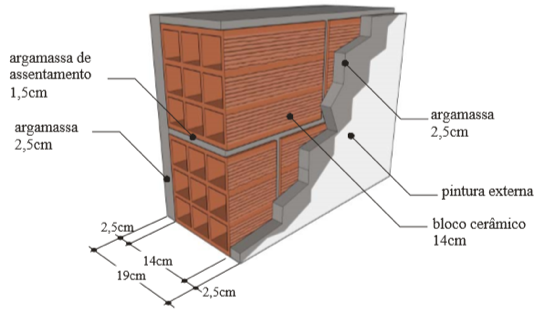
\includegraphics[width=0.4\textwidth]{figures/tab11-fig1.png}}  &                                                                       &                                                               & \multirow{8}{*}{\makecell[l]{Argamassa interna \\ \footnotesize(2,5cm); \\Bloco cerâmico \\ \footnotesize(14,0 x 19,0 x 29,0 cm);\\ Argamassa externa \\ \footnotesize(2,5cm); \\Pintura externa (\(\alpha\)).}}                  \\
                                                                                    &                                                                       &                                                               &                                                                                                                                                                                               \\
                                                                                    &                                                                       &                                                               &                                                                                                                                                                                               \\
                                                                                    &                                                                       &                                                               &                                                                                                                                                                                               \\
                                                                                    & 1,85                                                                  & 161                                                           &                                                                                                                                                                                               \\
                                                                                    &                                                                       &                                                               &                                                                                                                                                                                               \\
                                                                                    &                                                                       &                                                               &                                                                                                                                                                                               \\
                                                                                    &                                                                       &                                                               &                                                                                                                                                                                               \\ \hline
    \multirow{9}{*}{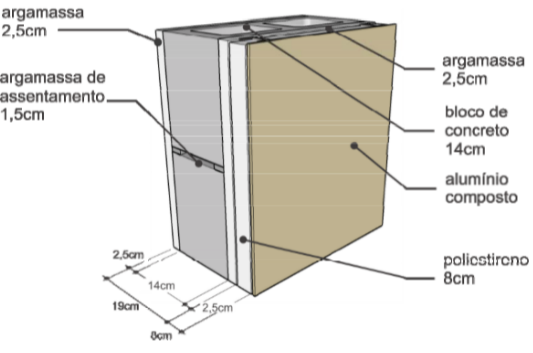
\includegraphics[width=0.4\textwidth]{figures/tab11-fig2.png}}  &                                                                       &                                                               & \multirow{9}{*}{\makecell[l]{Argamassa interna \\ \footnotesize(2,5 cm);\\ Bloco de concreto \\ \footnotesize(14,0 x 19,0 x 39,0 cm);\\ Argamassa externa \\ \footnotesize(2,5 cm);\\ Poliestireno \footnotesize(8 cm);\\ Placa de alumínio \\composto.}}  \\
                                                                                    &                                                                       &                                                               &                                                                                                                                                                                               \\
                                                                                    &                                                                       &                                                               &                                                                                                                                                                                               \\
                                                                                    &                                                                       &                                                               &                                                                                                                                                                                               \\
                                                                                    & 0,32                                                                  & 228                                                           &                                                                                                                                                                                               \\
                                                                                    &                                                                       &                                                               &                                                                                                                                                                                               \\
                                                                                    &                                                                       &                                                               &                                                                                                                                                                                               \\
                                                                                    &                                                                       &                                                               &                                                                                                                                                                                               \\
                                                                                    &                                                                       &                                                               &                                                                                                                                                                                               \\ \hline
    \multirow{9}{*}{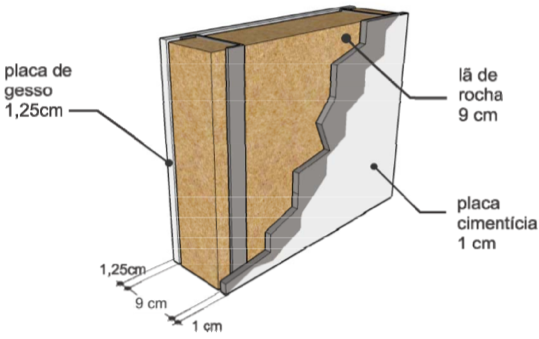
\includegraphics[width=0.4\textwidth]{figures/tab11-fig3.png}}  &                                                                       &                                                               & \multirow{9}{*}{\makecell[l]{Placa de gesso \\ \footnotesize(1,25 cm);\\ Lã de rocha \\ \footnotesize(9 cm);\\ Placa cimentícia \\ \footnotesize(1 cm).}}                                                                               \\
                                                                                    &                                                                       &                                                               &                                                                                                                                                                                               \\
                                                                                    &                                                                       &                                                               &                                                                                                                                                                                               \\
                                                                                    &                                                                       &                                                               &                                                                                                                                                                                               \\
                                                                                    & 0,38                                                                  & 269                                                           &                                                                                                                                                                                               \\
                                                                                    &                                                                       &                                                               &                                                                                                                                                                                               \\
                                                                                    &                                                                       &                                                               &                                                                                                                                                                                               \\
                                                                                    &                                                                       &                                                               &                                                                                                                                                                                               \\
                                                                                    &                                                                       &                                                               &                                                                                                                                                                                               \\ \hline
    \multicolumn{4}{c}{\textbf{Coberturas}}                                                                                                                                                                                                                                                                                                                                                                                 \\ \hline
    \multirow{6}{*}{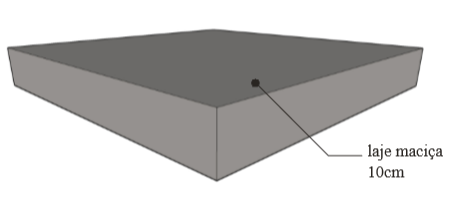
\includegraphics[width=0.4\textwidth]{figures/tab11-fig4.png}}  &                                                                       &                                                               & \multirow{5}{*}{\makecell[l]{Laje maciça \footnotesize(10 cm);\\ Sem telhamento.}}                                                                                                                         \\
                                                                                    &                                                                       &                                                               &                                                                                                                                                                                               \\
                                                                                    & 3,73                                                                  & 220                                                           &                                                                                                                                                                                               \\
                                                                                    &                                                                       &                                                               &                                                                                                                                                                                               \\
                                                                                    &                                                                       &                                                               &                                                                                                                                                                                               \\
                                                                                    &                                                                       &                                                               &                                                                                                                                                                                               \\ \hline
    \multicolumn{4}{c}{\textbf{Continua}}                                                                                                                                                                                                                                                                                                                                                                                   \\ \hline
\end{tabular}
\end{table} \pagebreak

\begin{table}[]
    \small
    \begin{tabular*}{\columnwidth}{@{\extracolsep{\fill}}lccl}
    \hline
    \multicolumn{4}{c}{\textbf{Conclusão}}                                                                                                                                                                                                                                                                                                                                                                                                  \\ \hline
    \multirow{9}{*}{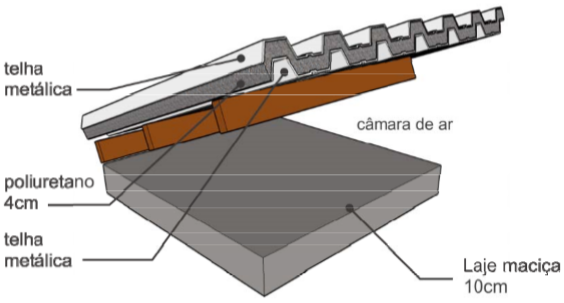
\includegraphics[width=0.4\textwidth]{figures/tab11-fig5.png}}  &                                                                       &                                            & \multirow{9}{*}{\makecell[l]{Laje pré-moldada (12 cm) \\(concreto 4 cm + EPS 7 cm + \\argamassa (1 cm);\\ Câmara de ar (\textgreater 5,0 cm);\\ Telha metálica (0,1 cm);\\ Poliuretano (4,0 cm);\\ Telha metálica (0,1 cm).}}    \\
                                                                                    &                                                                       &                                            &                                                                                                                                                                                                                                  \\
                                                                                    &                                                                       &                                            &                                                                                                                                                                                                                                  \\
                                                                                    &                                                                       &                                            &                                                                                                                                                                                                                                  \\
                                                                                    & 0,55                                                                  & 230                                        &                                                                                                                                                                                                                                  \\
                                                                                    &                                                                       &                                            &                                                                                                                                                                                                                                  \\
                                                                                    &                                                                       &                                            &                                                                                                                                                                                                                                  \\
                                                                                    &                                                                       &                                            &                                                                                                                                                                                                                                  \\
                                                                                    &                                                                       &                                            &                                                                                                                                                                                                                                  \\ \hline
    \multirow{9}{*}{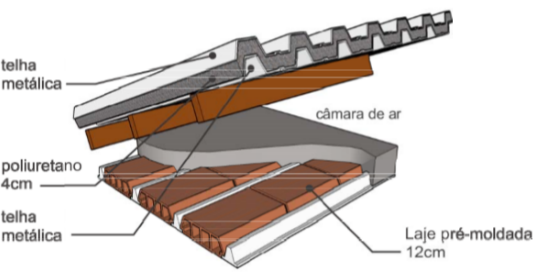
\includegraphics[width=0.4\textwidth]{figures/tab11-fig6.png}}  &                                                                       &                                            & \multirow{9}{*}{\makecell[l]{Laje maciça (10,0 cm);\\ Câmara de ar (\textgreater 5,0 cm);\\ Telha metálica (0,1 cm);\\ Poliestireno (isopor) (4,0 cm);\\ Telha metálica (0,1 cm).}}                                              \\
                                                                                    &                                                                       &                                            &                                                                                                                                                                                                                                  \\
                                                                                    &                                                                       &                                            &                                                                                                                                                                                                                                  \\
                                                                                    &                                                                       &                                            &                                                                                                                                                                                                                                  \\
                                                                                    & 0,53                                                                  & 176                                        &                                                                                                                                                                                                                                  \\
                                                                                    &                                                                       &                                            &                                                                                                                                                                                                                                  \\
                                                                                    &                                                                       &                                            &                                                                                                                                                                                                                                  \\
                                                                                    &                                                                       &                                            &                                                                                                                                                                                                                                  \\
                                                                                    &                                                                       &                                            &                                                                                                                                                                                                                                  \\ \hline
    \end{tabular*}
    \begin{flushleft}
        \par \small Fonte: autor (2019).\vspace{-0.6cm}
    \end{flushleft}
    \end{table}

\noindent A mudança de composição de vidro baseou-se na melhoria do desempenho energético para as zonas térmicas, onde a transmissão de radiação solar para o interior dos ambientes fosse mitigada, sem prejudicar o aproveitamento de luz natural \cite{CentroBrasileirodeEficienciaEnergeticaemEdificacoesCB3E2015,AssociacaoBrasileiradeNormasTecnicas-ABNT2013a,InstitutoNacionaldeMetrologiaNormalizacaoeQualidadeIndustrial-INMETRO2013,Ferreira2017} INSTITUTO..., 2013). Para tal, foi adotado o modelo mais eficiente, com baixa emissividade, como destacado na Tabela \ref{tab:tabela12}.
\begin{table}[H]
    \centering
    \small
    \caption{Propriedades físicas dos vidros adotados para os modelos genéricos.}
    \label{tab:tabela12}
    \begin{tabular}{lll}
    \hline
    \multicolumn{3}{c}{\textbf{Propriedade dos vidros}}                            \\ \hline
    \textbf{Fabricante}                      & CEBRACE          & CEBRACE          \\ \hline
    \textbf{Nome}                            & Reflecta Incolor & COOL-LITE ST 108 \\ \hline
    \textbf{Espessura}                       & 8 mm             & 6 mm             \\ \hline
    \textbf{Transmitância solar}             & 0,350            & 0,064            \\ \hline
    \textbf{Refletância solar externa (1)}   & 0,350            & 0,381            \\ \hline
    \textbf{Refletância visível interna (2)} & 0,340            & 0,485            \\ \hline
    \textbf{Transmitância visível}           & 0,320            & 0,078            \\ \hline
    \textbf{Refletância visível externa (1)} & 0,480            & 0,444            \\ \hline
    \textbf{Refletância visível interna (2)} & 0,510            & 0,377            \\ \hline
    \textbf{Emissividade externa (1)}        & 0,840            & 0,837            \\ \hline
    \textbf{Emissividade interna (2)}        & 0,840            & 0,147            \\ \hline
    \textbf{Condutividade}                   & 1,000            & 1,000            \\ \hline
    \textbf{Processo}                        & Laminado Incolor & Monolítico       \\ \hline
    \textbf{Transmitância ou U-value}        & 5,700            & 3,608            \\ \hline
    \textbf{Fator Solar ou SHGC}             & 0,440            & 0,160            \\ \hline
    \end{tabular}
    \begin{flushleft}
        \par \small Fonte: autor (2019).
    \end{flushleft}
    \end{table}
\vspace{-0.3cm} \noindent O PAF\textsubscript{T} foi implementado, variando entre 30\%, 50\% e 80\%, com a finalidade de evidenciar a influência sobre o consumo de energia relacionado às dimensões das aberturas e a área opaca das fachadas. Por relacionar componentes como a parede e o vidro, é um parâmetro de grande importância para o processo de determinação da eficiência energética.
\noindent Foram dimensionadas as proteções solares para cada um dos modelos, com base na incidência de orientação solar das edificações levantadas e no nível de obstrução vertical observado. Com o objetivo de bloquear a radiação solar direta presente nos horários mais quentes do dia, foram propostos brises fixos horizontais sobre as fachadas dos modelos genéricos entre os horários de 9 horas até às 16 horas. A escolha destes horários e a incidência de radiação solar direta é baseada em estudos de Hensen e Lamberts \citeyear{Hensen2012}.
\begin{figure}[H]
    \centering
    \caption{Detalhe da proteção solar de 1 m de comprimento da fachada oeste (a); carta solar da proteção solar de 1m (b)}
    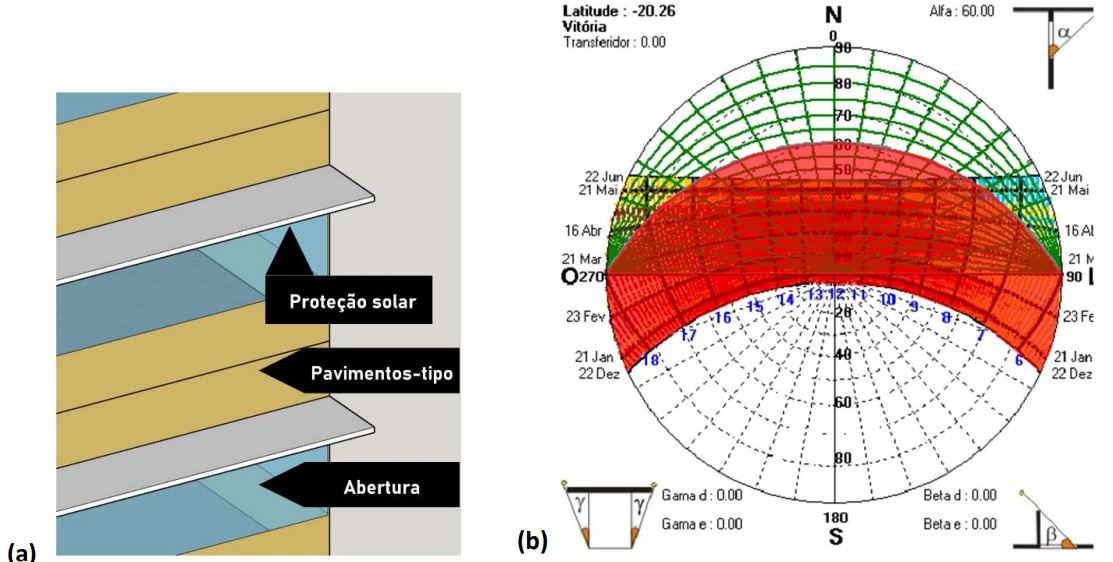
\includegraphics[width=1\textwidth]{figures/fig11-protecaosolar.jpg}
    \begin{flushleft}
        \par \small Fonte: autor (2019)
    \end{flushleft}
    \label{fig:figura12}
\end{figure}